\chapter{Generating molecules in the latent space of generative models}
\label{chapter:lso}

\ifpdf
    \graphicspath{{chapter0x-LSO/figures}}
\else
    \graphicspath{}
\fi

\newacronym{dgm}{DGM}{deep generative model}
\newacronym{lmo}{LSO}{latent space optimisation}
\newacronym{vae}{VAE}{variational autoencoder}
\newacronym{gan}{GAN}{generative adversarial network}
\newacronym{rl}{RL}{reinforcement learning}
\newacronym{bo}{BO}{Bayesian optimisation}
\newacronym{sgp}{SGP}{sparse Gaussian process}

\newcommand{\codelink}{\url{https://github.com/cambridge-mlg/weighted-retraining}
}
\newcommand{\bestchemscore}{27.84}

This chapter presents an approach
to Bayesian optimisation in molecule space,
originally published as
a conference paper in NeurIPS 2020 \citep{tripp2020sample}.
This conference paper was jointly written with
my supervisor José Miguel Hernández-Lobato
and fellow PhD student Erik Daxberger.
I had the original idea for this project
and conducted experiments jointly with Erik.
All three of us co-wrote the manuscript.

\section{Motivation}
\label{sec:lso:motivation}

Solving molecule optimisation problems (\S\ref{sec:background:molopt})
with \gls{bo} (\S\ref{sec:background:bayesopt}) poses two challenges
above and beyond BO in $\R^n$:

\begin{enumerate}
    \item The search space ($\amolspace$) is discrete,
        impeding the use of gradient-based methods to optimise the acquisition function
        $\alpha$ in line~\ref{alg:bo:maximise acqn fn} of algorithm~\ref{alg:general-bayesopt}.
    \item A probabilistic model over input graphs $p(\hat f)$
        must be created in line~\ref{alg:bo:fit model} of algorithm~\ref{alg:general-bayesopt},
        and there are arguably fewer options for such models in graph space.
\end{enumerate}
Moreover, these challenges are not unique to molecules:
any optimisation problem in a large and non-Euclidean input space will face similar challenges
(e.g.\@ design of protein sequences, designing neural network architectures).

One potential approach to tackle both challenges
is to perform optimisation over the latent variable of a generative model,
which we will refer to as \emph{\gls{lmo}}.
This approach has been proposed and used by many recent works
\citep{gomez2018,kusner_grammar_2017,lu2018structured,eismann_bayesian_2018,luo2018neural,kajino_molecular_2019,nguyen_synthesizing_2016,dai_syntax-directed_2018,daxberger2019bayesian,griffiths_constrained_2020,mahmood_cold_2019,antoran_getting_2020}.
We will give a brief overview of \gls{lmo} below.

Let $\X$ denote a general input space (e.g.\@ $\molspace$),
$\Z$ denote some \emph{latent space},
and $f:\X\mapsto\R$ denote an optimisation objective.
\Gls{lmo} first requires defining a \emph{\gls{dgm}}
$g: \Z\mapsto\X$ 
and a \emph{latent objective model} $\hat f: \Z\mapsto\R$
to approximate $f$ at the output of $g$, namely $f(g(\z))\approx \hat f(\z),\ \forall \z\in\Z$.
As part of this process,
an approximate inverse to $g$, $q:\X\mapsto\Z$
may be created to encode a set of known data points in $\X$ into $\Z$.
Then, the acquisition function $\alpha$
is optimised over $\Z$ instead of $\X$.
When a point $\bm{z}^*$ is chosen,
it is ``decoded'' into $x^*:=g(\bm{z}^*)$ in order to be evaluated.
Note that in this chapter we consider \emph{noiseless} evaluation,
i.e.\@ $y_i=f(x_i)$.
The potential advantage of \gls{lmo} is that $\Z$ can be continuous and low-dimensional (e.g.\@ $\R^n$),
making defining $\hat f$ and optimising acquisition functions easier.

Many prior works using \gls{lmo} apply it in a \textit{post-hoc} manner
by training a generative model decoupled from any optimisation task.
The first contribution in this chapter
a conceptual argument of why such decoupling may limit the performance of \gls{lmo} methods
(\S\ref{sec:lso:limitations}).
The second contribution of this chapter is a method desired to overcome these limitations
by combining dataset weighting and periodic retraining of the generative model (\S\ref{sec:lso:main}).
Finally, we show that this
method produces promising results on several empirical benchmarks (\S\ref{sec:lso:experiments}).


\section{Failure Modes of Latent Space optimisation}
\label{sec:lso:limitations}
To understand the shortcomings of \gls{lmo},
it is necessary to first examine in detail the role of the generative model, which is usually a \gls{dgm}.
State-of-the-art \glspl{dgm} such as \glspl{vae} and \glspl{gan}
are trained with a prior $p(\z)$ over the latent space $\Z$.
This means that although the resulting function $g:\Z\mapsto\X$ is defined over the entire latent space $\Z$,
it is effectively only trained on points in regions of $\Z$ with high probability under $p$.
Importantly, even if $\Z$ is an unbounded space with infinite volume such as $\mathbb{R}^n$,
because $p$ has finite volume, there must exist a \emph{finite} subset $\Z'\subset\Z$ that contains virtually all the probability mass of $p$.
We call $\Z'$ the \emph{feasible region} of $\Z$.
Although in principle optimisation can be performed over all of $\Z$,
it has been widely observed that optimising outside of the feasible region tends to give poor results,
yielding samples that are low-quality, or even invalid (e.g.\@ invalid molecular strings, non-grammatical sentences);
therefore all \gls{lmo} methods known to us employ some sort of measure to restrict the optimisation to near or within the feasible region
\citep{gomez2018,kusner_grammar_2017,nguyen_synthesizing_2016,griffiths_constrained_2020,white_sampling_2016,mahmood_cold_2019,daxberger2019bayesian}.
This means that \gls{lmo} should be treated as a \emph{bounded} optimisation problem,
whose feasible region is determined by $p$.

Informally, the training objective of $g$ encourages points sampled from within the feasible region to match the data distribution that $g$
was trained on, effectively ``filling'' the feasible region with points similar to the dataset,
such that a point's relative volume is roughly proportional to its frequency in the training data.
For many optimisation problems, most of the training data for the \gls{dgm} is low-scoring
(i.e.\@ highly suboptimal objective function values),
thereby causing most of the feasible region to contain low-scoring points.
Not only does this make the optimisation problem more difficult to solve (like finding the proverbial ``needle in a haystack''),
but actually leaves insufficient space in the feasible region for a large number of novel, high-scoring points that lie outside the training distribution to be modelled by the \gls{dgm}.
Therefore, even a perfect optimisation algorithm with unlimited evaluations of the objective function
might be unable to find a novel point
that is substantially better than the best point in the original dataset,
simply because such a point may not exist in the feasible region.

\begin{figure}
    \centering
    \begin{subfigure}[c]{0.245\textwidth}
        \centering
        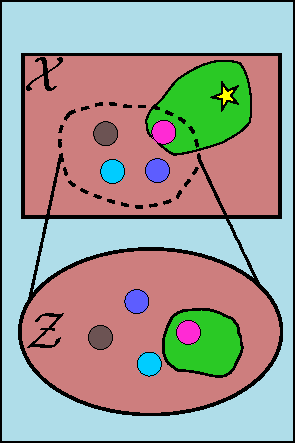
\includegraphics[width=0.9\textwidth]{schematic/base-v3.pdf}
        \vspace{-5mm}
        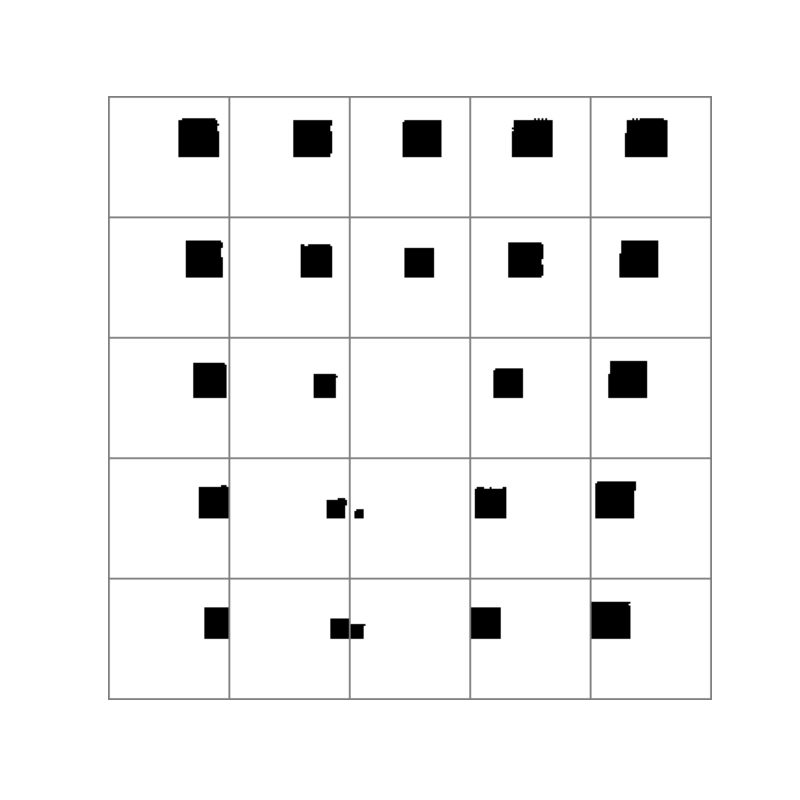
\includegraphics[width=0.95\textwidth]{schematic/shapes-manifold-plain.png}
        \subcaption{Starting Point}
        \label{subfig:lso-schematic-a}
    \end{subfigure}
    \begin{subfigure}[c]{0.245\textwidth}
        \centering
        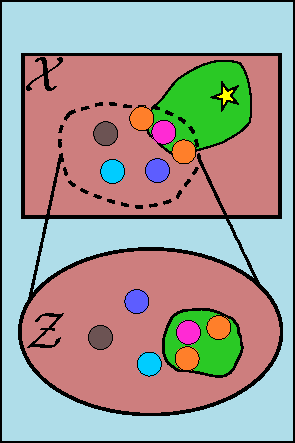
\includegraphics[width=0.9\textwidth]{schematic/normal-lso-res.pdf}
        \vspace{-5mm}
        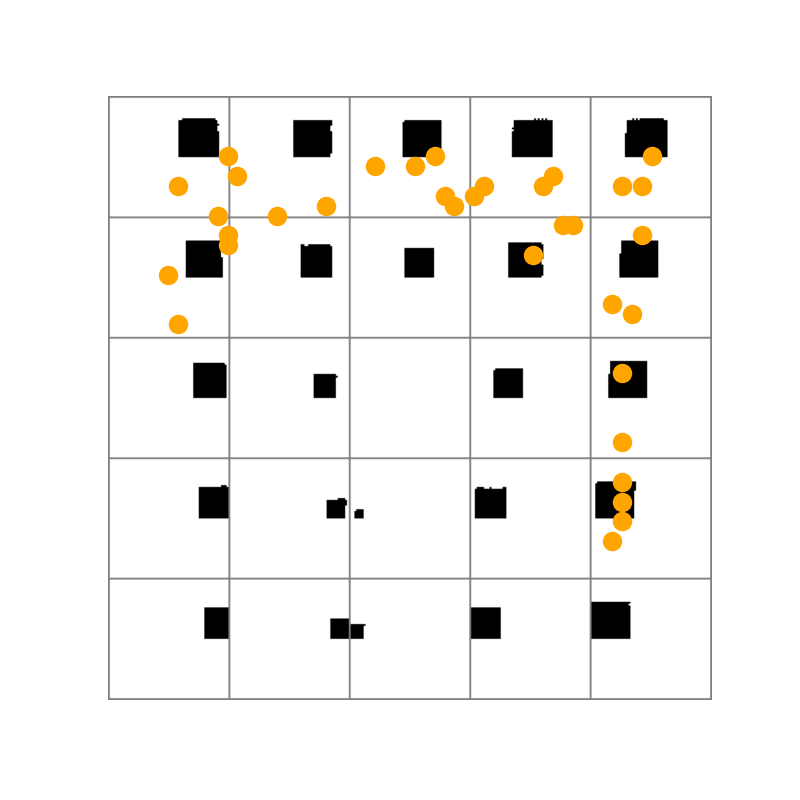
\includegraphics[width=0.95\textwidth]{schematic/shapes-manifold-plain-data.png}
        \subcaption{Standard \gls{lmo}}
        \label{subfig:lso-schematic-b}
    \end{subfigure}
    \begin{subfigure}[c]{0.49\textwidth}
        \centering
        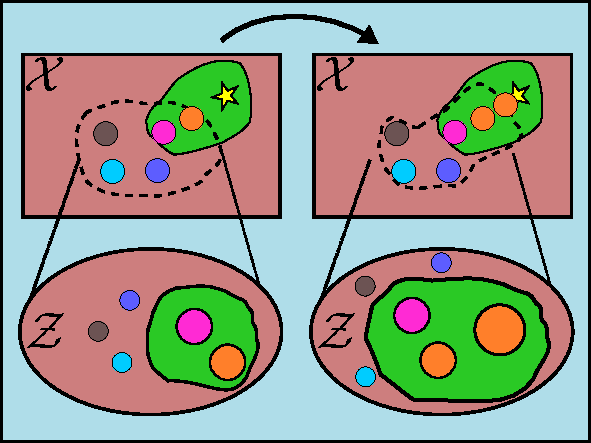
\includegraphics[width=0.9\textwidth]{schematic/wr-res.pdf}
        \vspace{-5mm}
        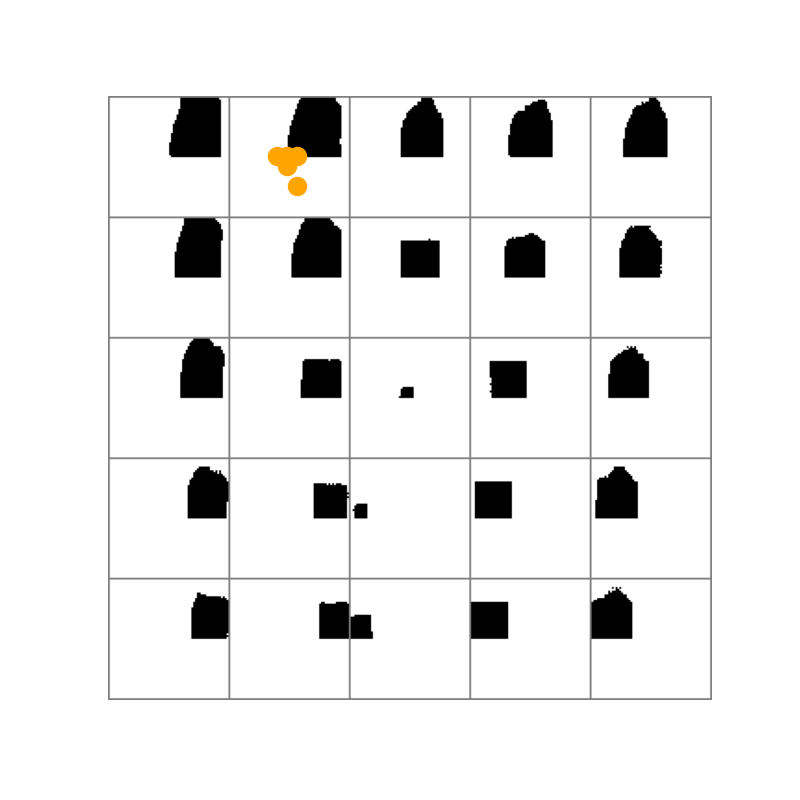
\includegraphics[width=0.475\textwidth]{schematic/shapes-manifold-wr-1.png}
        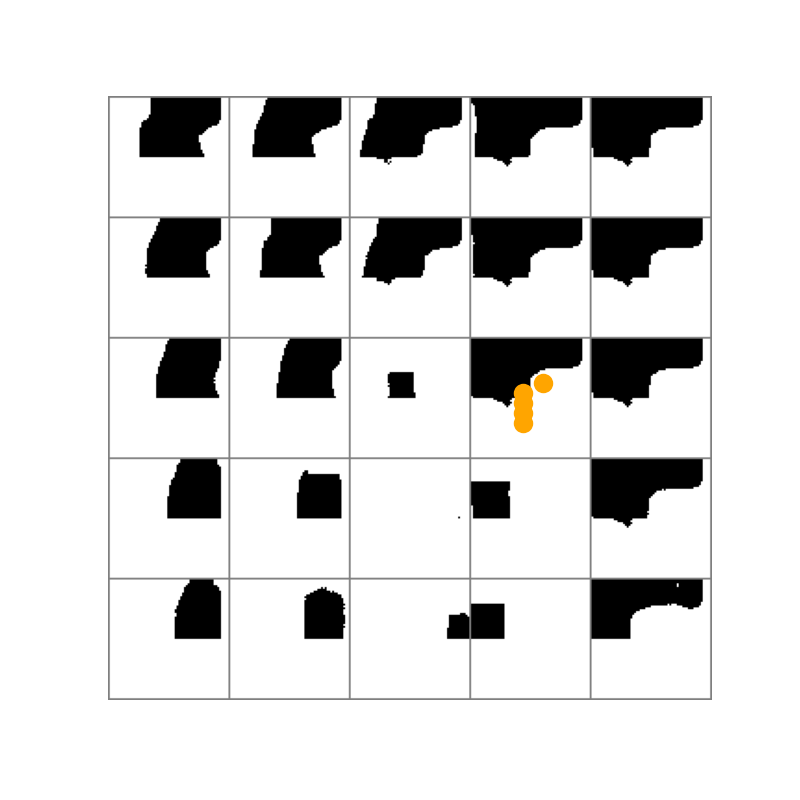
\includegraphics[width=0.475\textwidth]{schematic/shapes-manifold-wr-2.png}
        \subcaption{\Gls{lmo} with Weighted Retraining}
        \label{subfig:lso-schematic-c}
    \end{subfigure}
    \caption[Cartoon schematic of \gls{lmo}.]{
    Schematic illustrating \gls{lmo} with and without weighted retraining.
    The cartoon illustrates the input/latent space  of the generative model (\textbf{top}).
    The latent manifold from \cref{subsec:expt-wr}'s 2D shape area maximisation task is shown
    for comparison (\textbf{bottom}).
    Each image in the manifold shows the result of decoding a latent point on a uniform square grid in a 2D latent space;
    images are centred on the original grid points.
    Red/green regions correspond to points with low/high objective function values respectively.
    The yellow star is the global optimum in $\X$.
    Coloured circles are data points; their radius represents their weight.
    The dashed line surrounds the region of $\X$ modelled by $g$ (i.e.\@ $g(\Z)$, the image of $\Z$).
    \textbf{(a)} The status of the generative model $g$ at the start of optimisation.
    \textbf{(b)} The result of standard \gls{lmo} with $g$ fixed, which queries the points in orange.
    It is only able to find points close to the training data used to learn $\Z$, resulting in slow and incomplete exploration of $\mathcal{X}$.
    \textbf{(c)} The result midway (left) and at the end (right) of \gls{lmo} with our proposed approach,
    which weights data points according to their objective function value and retrains $g$ to incorporate newly queried data.
    This continually adjusts $\Z$ to focus on modelling the most promising regions of $\X$,
    speeding up the optimisation and allowing for substantial extrapolation beyond the initial training data.
    }
    \label{fig:lso-chpater-schematic}
\end{figure}

This pathological behaviour is conceptually illustrated in \cref{subfig:lso-schematic-b},
where \gls{lmo} is unable to find or even approach the global optimum that lies far from the training data.
We propose that \gls{lmo}'s performance is severely limited by two concrete problems in its setup.
The first problem is that the generative model's training objective (to learn a latent space that captures the data distribution as closely as possible),
does not necessarily match the true objective (to learn a latent space that is amenable to efficient optimisation of the objective function).
Put in terms of the cartoon in \cref{subfig:lso-schematic-b}, the feasible region that is learned, which uniformly and evenly surrounds the data points,
is not the feasible region that would be useful for optimisation,
which would model more of the green region at the expense of the red region.
This is also seen in the 2D shape area maximisation task (described in \S\ref{sec:lso:expt-tasks}).
In \cref{subfig:lso-schematic-b},
the latent manifold contains only low-area shapes that the model was trained on,
and nothing close to the all-black global optimum.
The second problem is that information on new points acquired during the iterative optimisation procedure
is not propagated to the generative model,
where it could potentially help to refine and expand the coverage of the feasible region,
uncovering new promising regions that an optimisation algorithm can exploit.
In terms of \cref{subfig:lso-schematic-b},
the new data is not used to shift the feasible region toward the green region, despite the optimisation process indicating that this is a very promising region of $\X$ for optimisation.
Luckily, we believe that neither of these two problems is inherent to \gls{lmo}, and now pose a framework that directly addresses them.

\section{Latent Space optimisation with Weighted Retraining}
\label{sec:lso:main}
\subsection{Training a Generative Model with a Weighted Training Objective}
\label{subsec:weighting}
While it is unclear in general how to design a generative model that is maximally amenable to \gls{lmo},
the argument presented in \cref{sec:lso:limitations} suggests that it would at least be beneficial to dedicate
a higher fraction of the feasible region to modelling high-scoring points.
One obvious but inadequate method of achieving this is to simply discard all low-scoring points from the dataset used to train the \gls{dgm}, e.g.\@ by keeping only the top 10\% of the data set (in terms of score).
While this strategy could be feasible if data is plentiful, when data is scarce this option may not be viable
because state-of-the-art neural networks need a large amount of training data to avoid overfitting.
This issue can be resolved by not viewing inclusion in the dataset as a binary choice,
but instead as a \emph{continuum} that can be realized by \emph{weighting} the data points unevenly.
If the generative model is trained on a distribution that systematically places more probability mass on high-scoring points
and less mass on low-scoring points,
the distribution-matching term in the \gls{dgm}'s training objective will incentivize a larger fraction of the feasible
region's volume to be used to model high-scoring points,
while simultaneously using all known data points to learn useful representations and avoid overfitting.

A simple way to achieve this weighting is to assign an explicit weight $w_i\in[0,1]$ to each data point, such that $\sum_i w_i=1$.
As the training objective of common \glspl{dgm} involves the expected value of a loss
function $\mathcal{L}$ with respect to the data distribution,%
\footnote{For a \gls{vae}, $\mathcal{L}$ is the per-data point ELBO \citep{kingma2013auto}, while for a \gls{gan}, $\mathcal{L}$ is the discriminator score \citep{goodfellow2014generative}.}
weighted training can be implemented by simply replacing the empirical mean over the training data with a \emph{weighted} empirical mean:
i.e.\@ $\sum_{\x_i \in \D} w_i\mathcal{L}(\x_i)$ instead of $\sum_{\x_i \in \D} \frac{1}{N} \mathcal{L}(\x_i)$.
In practice, mini-batch stochastic gradient descent is used to optimise this objective
to avoid summing over all data points.
Unbiased mini-batches can be constructed by sampling each data point $\x_i$ with probability $w_i$
with replacement to construct each batch.

We offer no universal rules for setting weights, except that all weights $w_i$ should be restricted to strictly positive values,
because a negative weight would incentivize the model to perform poorly,
and a weight of zero is equivalent to discarding a point.
This aside, there are many reasonable ways to choose the weights such that high-scoring points are weighted more,
and low-scoring points are weighted less.
In this work, we decide to use a rank-based weight function,
\begin{equation}
\label{eq:weighting_function}
    w(\x; \D, k) \propto \frac{1}{kN + \text{rank}_{f,\D}(\x)}, \quad \text{rank}_{f,\D}(\x) = \left|\left\{\x_i : f(\x_i) > f(\x),\ \x_i \in \D \right\}\right|\ ,
\end{equation}
which assigns a weight roughly proportional to the reciprocal (zero-based) rank of each data point.
We chose \cref{eq:weighting_function} because it yields weights which are always positive,
resilient to outliers by virtue of using ranks, and will behave similarly over a range of dataset sizes.
Furthermore, as shown in \cref{fig:weighting}, it admits a single tunable hyperparameter $k\in(0,\infty)$ which continuously controls the degree of weighting,
where $k\to\infty$ corresponds to uniform weighting, i.e.\@ $w_i = \frac{1}{N}, \forall i$, while $k\to0$ places \emph{all} mass on only the single point with the highest objective function value.

\begin{figure}[ht]
    \centering
    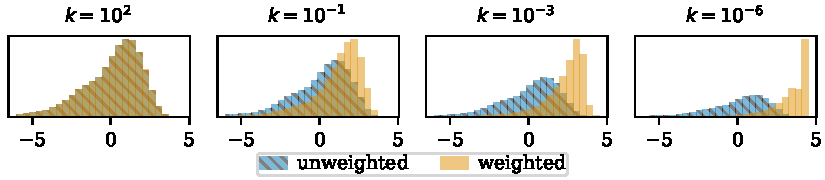
\includegraphics{histograms/train-data-hist-chem.pdf}
    \caption[Histogram of objective function values for the ZINC dataset]{
    Histogram of objective function values for the ZINC dataset (see \cref{sec:lso:experiments})
    with uniform weighting (in blue) as well as rank weighting from \cref{eq:weighting_function} for different $k$ values (in orange).
    Large $k$ approaches uniform weighting, while small $k$ places most weight on high-scoring points.
    }
    \label{fig:weighting}
\end{figure}

\subsection{Periodic Retraining to Update the Latent Space}
\label{subsec:retraining}
To allow the latent manifold to adapt to new information,
we propose a conceptually simple solution: \emph{periodically retraining the generative model} during the optimisation procedure.
In practice, this could be done by training a new model from scratch,
or by fine-tuning the previously trained model on the novel data.
However, as is often pointed out in the active learning literature,
the effect of adding a few additional points to a large dataset is rather negligible,
and thus it is unlikely that the generative model will change significantly if retrained on
this augmented dataset \citep{sener_active_2018}.
While one could also retrain on \emph{only} the new data,
this might lead to the well-known phenomenon of catastrophic forgetting \citep{mccloskey_catastrophic_1989}.

A key observation we make is that \emph{the data weighting outlined in \cref{subsec:weighting} actually resolves this problem}.
Specifically, if the new points queried are high-scoring,
then a suitable weighting scheme (such as \cref{eq:weighting_function}) will assign a large weight to them,
while simultaneously decreasing the weights of many of the original data points,
meaning that a small number of new points can have a disproportionate impact on the training distribution.
If the generative model is then retrained using this distribution,
it can be expected to change significantly to incorporate these new points into the latent space in order to minimise the weighted loss.
By contrast, if the new points queried are low-scoring,
then the distribution will change negligibly, and the generative model will not significantly update, thereby avoiding adding new low-scoring points into the feasible region.
\subsection{Weighted Retraining Combined}
\label{subsec:weighted-retraining}
When put together, \emph{data weighting} and \emph{periodic retraining} complement each other elegantly,
transforming the generative model from a passive decoding function into an active participant
in the optimisation process,
whose role is to ensure that the latent manifold is constantly
occupied by the most updated and relevant points for optimisation.
Their combined effect is visualized conceptually in \cref{subfig:lso-schematic-c}.
In the first iteration, weighted training creates a latent space with more high scoring points,
causing the feasible region to extend farther into the green region at the expense of the red region.
This allows a better orange point to be chosen relative to \cref{subfig:lso-schematic-b}.
In the second iteration in \cref{subfig:lso-schematic-c},
weighted training with the orange point 
incorporates even more high-scoring points into the latent space,
allowing an even better point to be found.
Qualitatively similar results can be seen in the 2D shape area maximisation task,
where weighted retraining introduces points with very high areas
into the latent space compared to \cref{subfig:lso-schematic-a}
(details for this experiment are given in \cref{sec:lso:experiments}).

\begin{algorithm}[tb]
\caption{Latent Space optimisation {\color{blue} with Weighted Retraining} (changes highlighted in {\color{blue} blue}).}
\label{alg:lso-weighted-retraining}
\begin{algorithmic}[1]
    \STATE {\bfseries Input:} Data $\D = \{(\x_i, f(\x_i))\}_{i=1}^N$, query budget $M$, objective function $f(\x)$, latent objective model $\hat f(\z)$,
    generative/inverse model $g(\z)$/$q(\x)$, {\color{blue} retrain frequency $r$, weighting function $w(\x)$}
    \vspace{1mm}
    {\color{blue}\FOR{$1, \ldots, M$\textcolor{blue}{$/r$}}
        {\color{black} \STATE Train generative model $g$ and inverse model $q$ on data $\D$ {\color{blue} weighted by $\mathcal{W} = \{w(\x)\}_{\x \in \D}$}%
        \vspace{1mm}
    	\FOR{$1, \ldots, $\textcolor{blue}{$r$}}
            \STATE Compute latent variables $\mathcal{Z} = \{\z = q(\x)\}_{\x \in \D}$
            \STATE Fit objective model $\hat f$ to $\mathcal{Z}$ and $\D$,
            and optimise $\hat f$
            to obtain new latent query point $\tilde{\z}$
    	    \STATE Obtain corresponding input $\tilde{\x} = g(\tilde{\z})$, evaluate $f(\tilde{\x})$ and set $\D \gets \D \cup \{(\tilde{\x}, f(\tilde{\x}))\}$
        \ENDFOR}
    \ENDFOR}
    \vspace{1mm}
	\STATE {\bfseries Output:} Augmented dataset $\D$
\end{algorithmic} 
\end{algorithm}

In the remainder of this chapter, we refer to the combination of these techniques as
\emph{weighted retraining} for brevity; see \cref{alg:lso-weighted-retraining} for pseudocode.
Computationally, the overhead of the weighting is minimal, and the cost of the retraining
can be reduced by fine-tuning an existing model on the weighted dataset instead of retraining it from scratch.
Although this may still be prohibitively expensive for some applications,
we stress that in many scenarios the cost of training a model is insignificant compared to even a single evaluation of the objective function (e.g.\@ performing wet-lab experiments for drug design),
making weighted retraining a sensible choice.

\section{Related Work}
\label{sec:lso:related-work}
In this section we compare and contrast 
our proposed latent space optimisation with weighed retraining
with other methods in the literature.

\subsection{Procedures analogous to weighted retraining}
A few previous machine learning methods can be viewed as implementing a version of weighted retraining.
The cross-entropy (CE) method iteratively retrains a generative model using a weighted training set,
such that high-scoring points receive higher weights \citep{rubinstein_optimization_1997,rubinstein_cross-entropy_1999,de2005tutorial}.
Indeed, particular instantiations of the CE method such as reward-weighted regression \citep{peters2007reinforcement},
feedback GAN \citep{gupta_feedback_2019},
and design/conditioning by adaptive sampling (DbAS/CbAS) \citep{Brookes_Listgarten_2020,brookes2019conditioning}
have been applied to similar problem settings as our work.
However, our proposed method of weighted retraining has two main differences from CE.
Firstly, \emph{standard CE produces only binary weights} \citep{de2005tutorial}, which amounts to simply adding or removing points from the training set.%
\footnote{Although methods such as DbAS \citep{Brookes_Listgarten_2020} generalize these weights to lie in $[0,1]$, this is determined by the noise of the oracle and therefore will still produce binary weights when $f$ is deterministic, as considered in this chapter.}
This is suboptimal for reasons discussed in \cref{subsec:weighting,subsec:retraining}, and consequently, \emph{we consider a strictly more general form of weighting}.
Secondly, \emph{CE has no intrinsic optimisation component.}
High-performing points are found only by repeatedly sampling from the generative model and evaluating $f$.
By contrast, our method \emph{explicitly selects high-performing points} using Bayesian optimisation.
The necessity of repeated sampling in CE makes it only suitable in cases where evaluating $f$ is cheap, which is \emph{not} what we are considering.
Moreover, works such as \citep{segler_generating_2018} perform optimisation by fine-tuning a generative model on a smaller dataset of high-scoring samples.
This can also be viewed as a special case of weighted retraining with binary weights,
where the weights are implicitly defined by the number of fine-tuning epochs.

\subsection{Bayesian optimisation}

Our method fits comfortably within the Bayesian optimisation framework (\S\ref{sec:background:bayesopt}).
It is effectively an input-agnostic procedure to create probabilistic models
and update them throughout the optimisation procedure.
Perhaps the most similar work to ours is \citet{blanchard_output_weighted_2020},
use a weighted \emph{acquisition function} to increase the sample efficiency of \gls{bo}
(although they do not use these weights to create the model itself).

\subsection{Reinforcement Learning}
\Gls{rl} frames optimisation problems as Markov decision processes for which an agent learns an optimal policy \citep{sutton1998introduction}.
It has recently been applied to various optimisation problems in structured input spaces \citep{li_deep_2018}
where we believe latent space optimisation with weighted retraining may be effective,
notably in chemical design \citep{you_graph_2018,zhou_optimization_2019,guimaraes_objective-reinforced_2018,olivecrona_molecular_2017,popova_deep_2018,simm_reinforcement_2020}.
While \gls{rl} is undoubtedly effective at optimisation, it is generally extremely sample inefficient,
and consequently its biggest successes are in virtual environments where function evaluations are inexpensive \citep{li_deep_2018}.

\subsection{Conditional Generative Models}
One interesting direction is the development of \emph{conditional generative models},
which directly produce novel points conditioned on a specific property value \citep{sohn_learning_2015,mirza_conditional_2014}.
Although many variants of these algorithms have been applied to real-world problems such as chemical design 
\citep{jin_learning_2019,kang_conditional_2019,li_multi-objective_2018,lim_molecular_2018,Brookes_Listgarten_2020},
the sample efficiency of this paradigm is currently unclear.

\section{Empirical Evaluation}
\label{sec:lso:experiments}
This section aims to empirically answer three main questions:
\begin{enumerate}
    \item How does weighted training affect the latent space of \glspl{dgm}? (\S\ref{subsec:expt-weighting})
    \item How do the parameters of weighted retraining influence optimisation? (\S\ref{subsec:expt-wr})
    \item Does weighted retraining compare favourably to existing methods? (\S\ref{subsec:expt-baselines})
\end{enumerate}
To answer these questions, we perform experiments using three optimisation tasks 
chosen to represent three different data and model types.
The tasks are described in \S\ref{sec:lso:expt-tasks}.
Because there is no obvious single metric to evaluate sample-efficient optimisation,
we choose to plot the $K$th best novel evaluated point as a function of the number of objective function evaluations,
which we denote as the \emph{Top$K$} score.
All plots show the average performance and standard deviation across runs with 5 different random seeds unless otherwise stated.
This evaluation method is common practice in Bayesian optimisation \citep{shahriari2015taking}.
It contrasts with previous works which typically report only final scores,
and take the maximum across seeds rather than the average
\citep{gomez2018,kusner_grammar_2017,dai_syntax-directed_2018,jin_junction_2019}.

All experimental data and code to reproduce the experiments can be found at 
\codelink{}.

\subsection{Tasks}
\label{sec:lso:expt-tasks}

\subsubsection{2D Shape Area Maximisation Toy Task}
As a simple toy task that can be easily visualized in 2D,
we optimise for the shape with the largest total area in the space of $64\times64$ binary images
(i.e.\@ the largest number of pixels with value 1).

\paragraph{Data} A dataset of $\approx$10,000 squares of different sizes and positions
on a $64\times64$ background, with a maximum area of 400
(see \cref{fig:shape-samples} for examples).
\paragraph{Model} A convolutional \gls{vae} with $\Z=\mathbb{R}^2$,
as a standard neural network architecture for image modelling.
It was implemented using PyTorch \citep{paszke2019pytorch} and PyTorch Lightning \citep{falcon2019pytorch}.
\paragraph{Latent optimiser} We enumerate a grid in latent space over $[-3,+3]^2$,
to emulate a perfect optimiser for illustration purposes (this is only feasible since $\Z$ is low-dimensional).

\begin{figure}[ht]
    \centering
    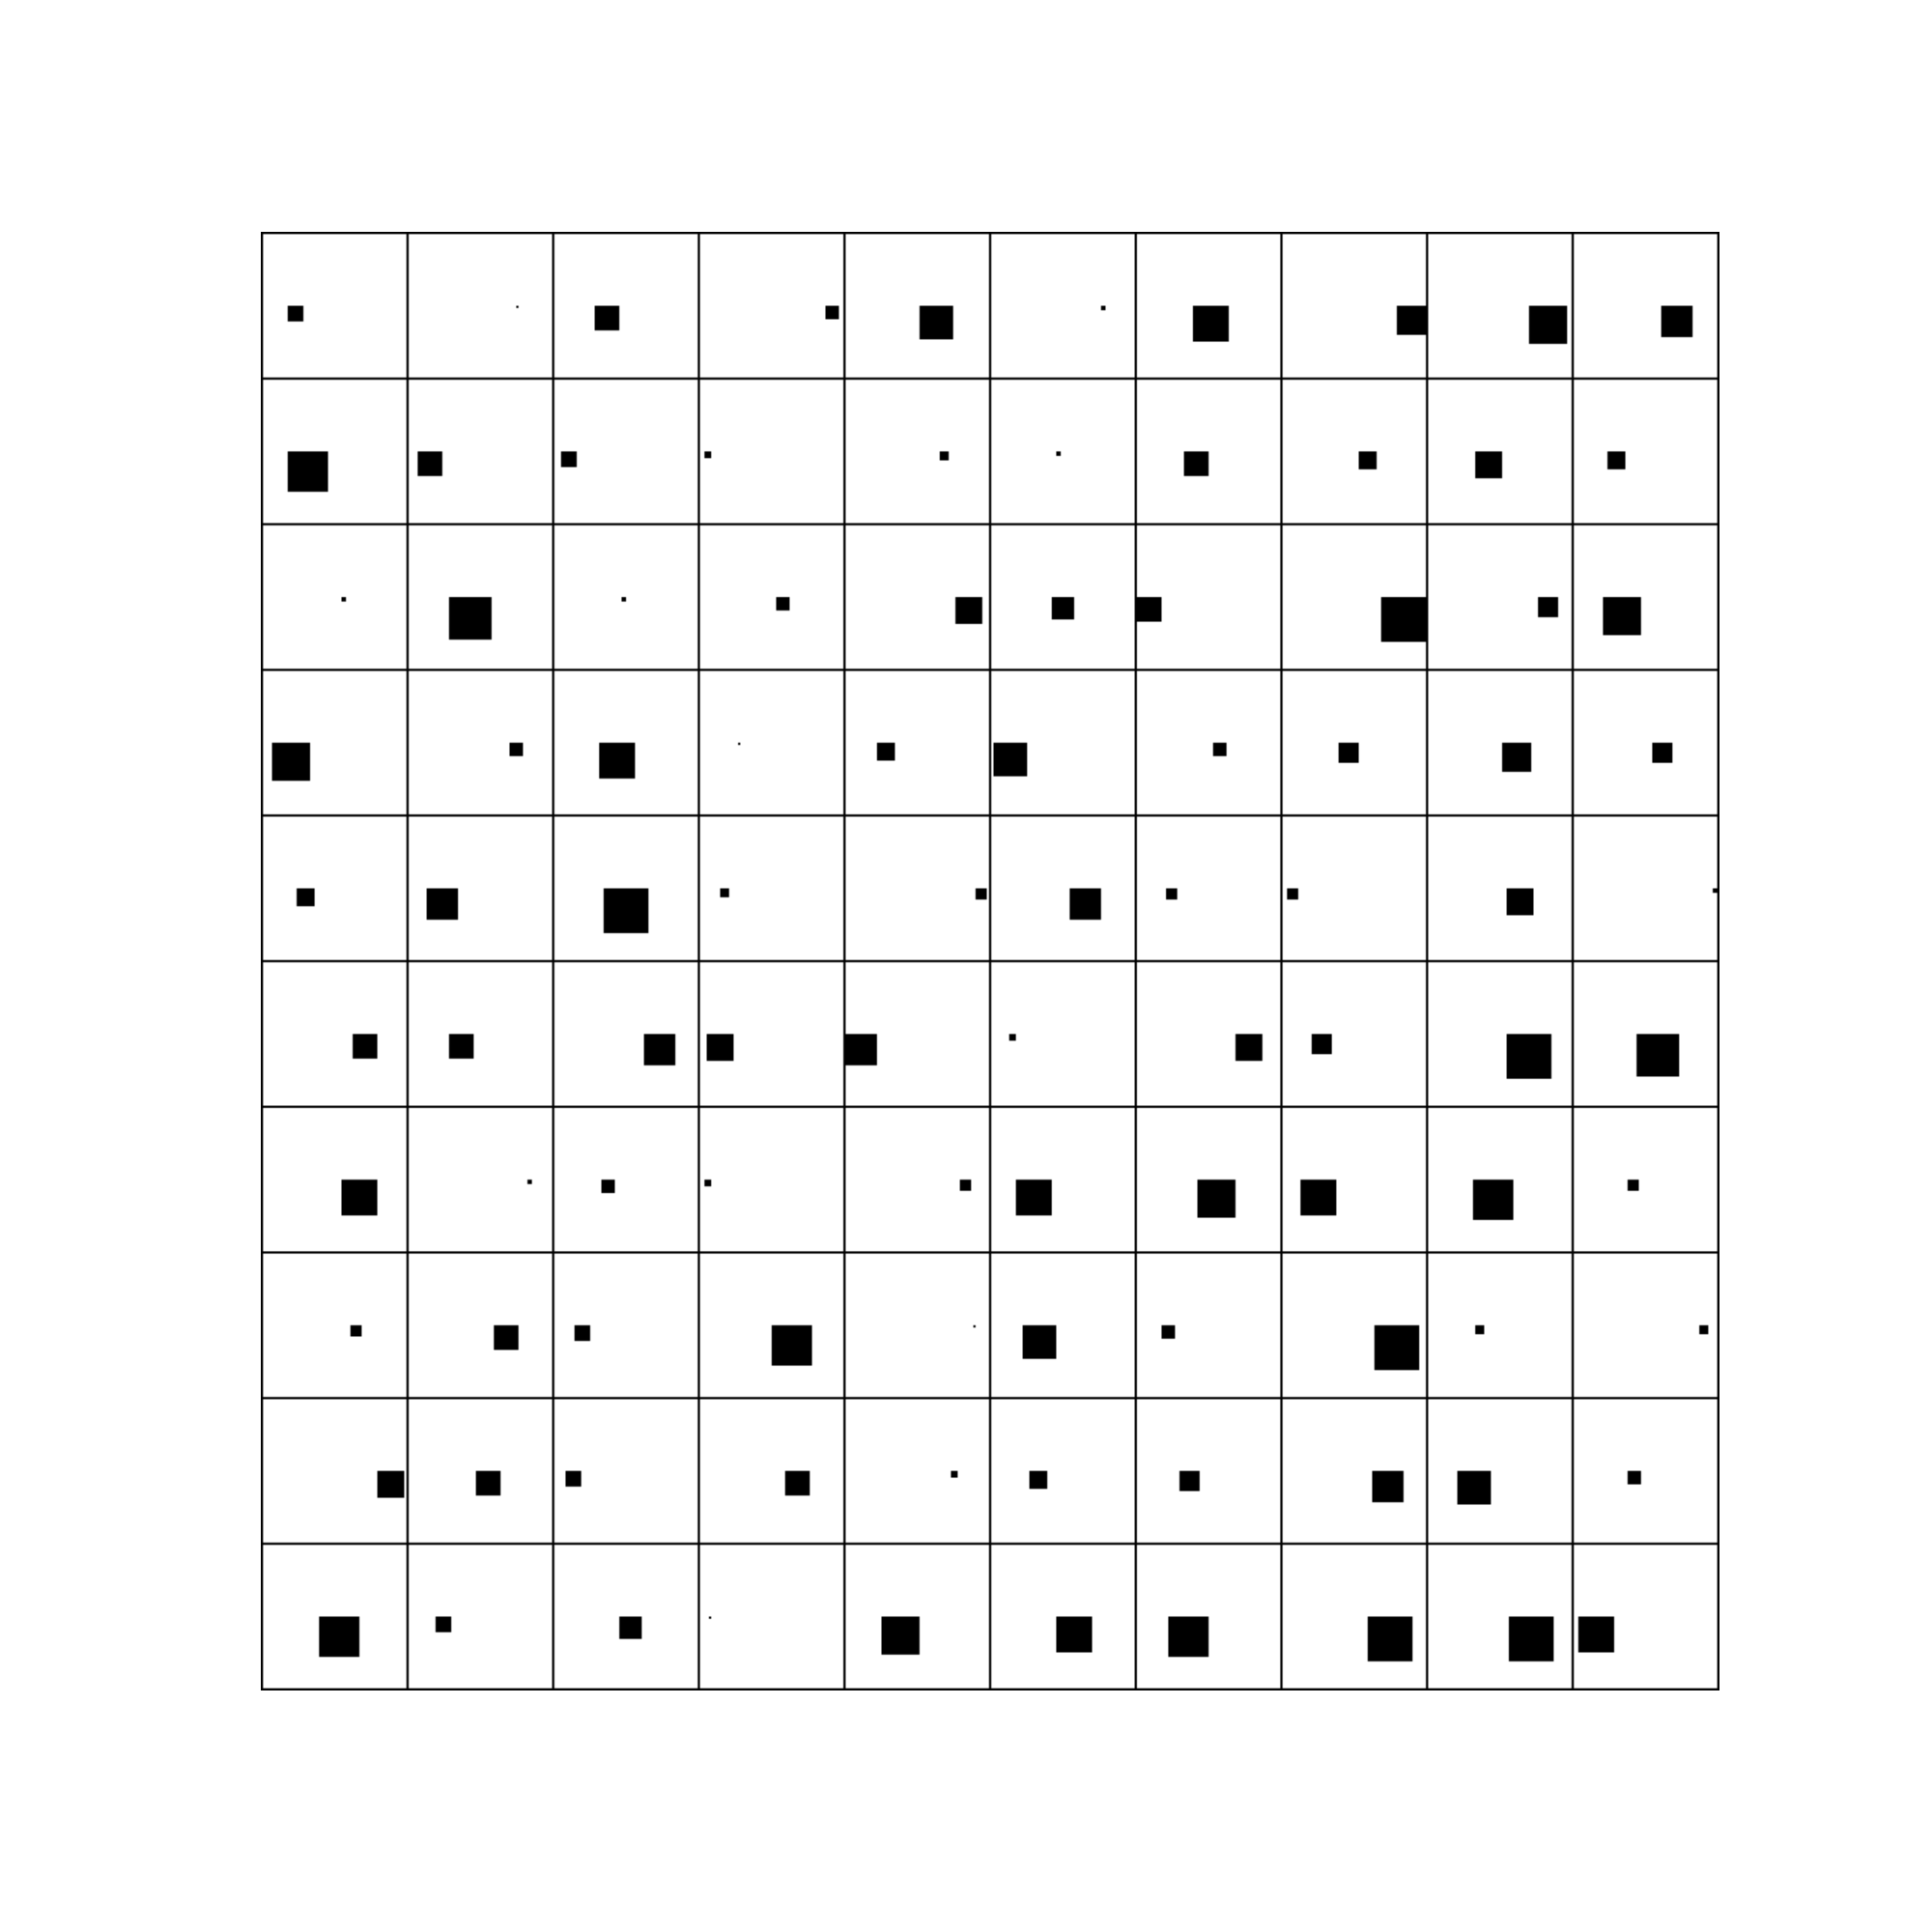
\includegraphics[width=0.6\textwidth]{shapes-train-data-samples.png}
    \caption{Sample images from our 2D squares dataset.}
    \label{fig:shape-samples}
\end{figure}

\subsubsection{Arithmetic Expression Fitting Task}
We follow \citet{kusner_grammar_2017} and optimise in the space of single-variable
arithmetic expressions generated by the formal grammar
\begin{align*}
    &\texttt{S $\rightarrow$ S '+' T | S '*' T | S '/' T | T}\\
    &\texttt{T $\rightarrow$ '(' S ')' | 'sin(' S ')' | 'exp(' S ')'}\\
    &\texttt{T $\rightarrow$ 'v' | '1' | '2' | '3'}\ ,
\end{align*}
where \texttt{S} and \texttt{T} denote non-terminals and the symbol \texttt{|}
separates the possible production rules generated from each non-terminal.
Every string in the dataset was generated by applying at most 15 production rules,
yielding arithmetic expressions such as \texttt{sin(2)}, \texttt{v/(3+1)} and \texttt{v/2 * exp(v)/sin(2*v)},
which are all considered to be functions of the variable \texttt{v}.
Following \citet{kusner_grammar_2017}, the objective is to find an expression
with minimal mean squared error to the target expression $\x^* = \texttt{1/3 * v * sin(v*v)}$,
computed over 1000 values of \texttt{v} evenly-spaced between $-10$ and $+10$.
In contrast to the original dataset of size 100,000 used by \citet{kusner_grammar_2017},
which \emph{includes the target expression} and many other well-performing inputs
(thus making the optimisation problem easy in theory), we make the task more challenging
by discarding the 50\% of points with the highest scores, resulting in a dataset of
size 50,000 with objective function value distribution shown in \cref{fig:weighting_equation}.
\paragraph{Data} 50,000 univariate arithmetic expressions generated by the formal grammar from \citet{kusner_grammar_2017}.
\paragraph{Model} A grammar \gls{vae} \citet{kusner_grammar_2017},
chosen because of its ability to produce only valid grammatical expressions.
Our implementation of the grammar \gls{vae} is based on the code from 
\citep{kusner_grammar_2017} provided at \url{https://github.com/mkusner/grammarVAE},
which we modified to use Tensorflow 2 \citep{abadi2016tensorflow} and python 3.
\paragraph{Latent optimiser} Bayesian optimisation with the expected improvement acquisition function \citep{jones1998efficient}
and a \glsfirst{sgp} model with 500 inducing points \citep{titsias2009variational},
following \citet{kusner_grammar_2017}.
We re-implemented the outdated and inefficient \texttt{Theano}-based Bayesian optimisation
implementation\footnote{see \url{https://github.com/mkusner/grammarVAE}}
of \citet{kusner_grammar_2017} (which was also used by \citep{jin_junction_2019})
using the popular and modern \texttt{Tensorflow 2.0}-based \texttt{GPflow} Gaussian process library
\citep{de2017gpflow} to benefit from GPU acceleration.
For computational efficiency, we fit the \gls{sgp} only on a subset of the data, consisting of the 2000 points
with the highest objective function values,
and 8000 randomly chosen points.
This also has the effect of ensuring that the \gls{sgp} properly fits the high-performing regions of the data.
Disregarding computational efficiency, we nonetheless found that fitting on this data subset remarkably improved performance
of the optimisation, even using the baseline model (without weighted retraining).

\begin{figure}[ht]
    \centering
    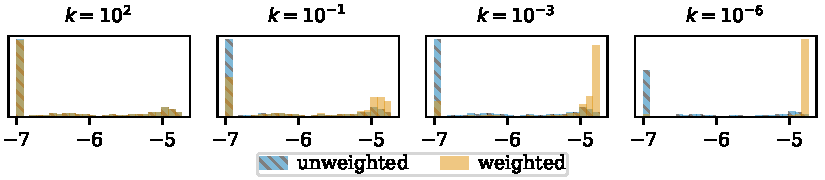
\includegraphics{histograms/train-data-hist-expr.pdf}
    \caption[Rank weighting on the arithmetic expression dataset.]{
    Illustration of rank weighting (\cref{eq:weighting_function})
    on the arithmetic expression dataset (defined in \cref{sec:lso:experiments}).
    }
    \label{fig:weighting_equation}
\end{figure}

\subsubsection{Chemical Design Task}
We follow \citet{gomez2018} and optimise the drug properties of molecules.
In particular, we consider the standardized task originally proposed in \citet{gomez2018}
of synthesizing a molecule with maximal penalized \emph{water-octanol partition coefficient} (logP),
starting from the molecules in the ZINC250k molecule dataset \citep{irwin_zinc_2012}.
The precise scoring function for a chemical $\x$ is defined as:
\begin{equation*}
\text{score}(\x) = \max\left(\widehat{\log{P}(\x)} -\widehat{\text{SA}(\x)} - \widehat{\text{cycle}(\x)}, \ -4\right)
\end{equation*}
where $\log{P}$, SA, and cycle are property functions,
and the $\ \widehat{}\ $ operation indicates standard normalization of the raw function output using the ZINC training set data
(i.e.\@ subtracting the mean of the training set, and dividing by the standard deviation).
This is identical to the scoring function from references \citep{kusner_grammar_2017,dai_syntax-directed_2018,jin_junction_2019,zhou_optimization_2019,you_graph_2018},
except that we bound the score below by $-4$ to prevent points with highly-negative scores from substantially impacting the optimisation procedure.
Functionally, because this is a maximisation task, this makes little difference to the scoring of the outcomes,
but does substantially help the optimisation.
This task has been studied in a long series of papers performing optimisation in chemical space,
allowing the effect of weighted retraining to be quantitatively compared to other optimisation approaches
\citep{kusner_grammar_2017,dai_syntax-directed_2018,jin_junction_2019,zhou_optimization_2019,you_graph_2018}.
\paragraph{Data} The ZINC250k molecule dataset \citep{irwin_zinc_2012}, using the same train/test split as \citep{jin_junction_2019}.
\paragraph{Model} A junction tree \gls{vae} \citep{jin_junction_2019},
chosen because it is a state-of-the-art \gls{vae} for producing valid chemical structures.
For direct comparability to previous results,
we use the pre-trained model provided in the code repository of \citep{jin_junction_2019} as the unweighted model,
and create weighted models by fine-tuning the pre-trained model for 1 epoch over the full weighted dataset.
\paragraph{Latent optimiser} Same as for the arithmetic expression task.


\subsection{Effect of Weighted Training}
\label{subsec:expt-weighting}
In this section, we seek to validate some of the conjectures made in \cref{sec:lso:limitations,sec:lso:main},
namely that 1) the latent space of a \gls{dgm} trained on uniformly weighted data contains many poor-performing points, and 2) that weighted training fixes this by introducing more high-performing points into the latent space.
To test this, we train a \gls{vae} for each task using rank weighting with a variety of $k$ values (noting that $k=\infty$ corresponds to uniform weighting), initializing the weights using a pre-trained \gls{vae} to ensure that the different runs are comparable.
We evaluate $f$ on samples from the \gls{dgm}'s prior for each task, and plot the resulting distributions in \cref{fig:prior-samples} with the label \emph{before retraining}.
Although the distribution of scores for $k=\infty$ does not exactly match the training distribution
for any example, it tends to have a similar range, showing that much of the latent space is dedicated to modelling low-scoring points.
Weighted training robustly causes the distribution to skew towards higher values at the expense of lower values, which is exactly the intended effect.
The upshot is that the result on all 3 tasks broadly supports our conjectures.

\begin{figure}[ht]
    \centering
    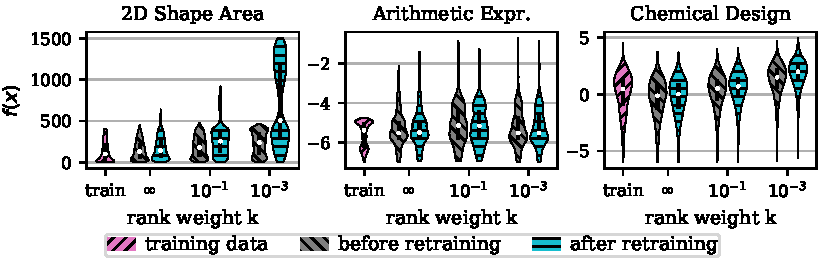
\includegraphics{violin.pdf}
    \caption[Prior samples from the \gls{dgm}'s prior for all tasks.]{
    Objective value distribution for the training set and samples from the \gls{dgm}'s prior
    for all three tasks for different $k$ values,
    before and after weighted retraining (see \cref{subsec:expt-wr}).
    }
    \label{fig:prior-samples}
\end{figure}


\subsection{Effect of Weighted Retraining Parameters on optimisation}
\label{subsec:expt-wr}
When using rank-weighting from \cref{eq:weighting_function} with parameter $k$ and picking a fixed period for model retraining $r$,
\gls{lmo} with weighted retraining can be completely characterized by $k$ and $r$.
The baseline of uniform weighting and no retraining is represented by $k=r=\infty$,
with decreasing values of $k$ and $r$ representing more skewed weighting and more frequent retraining, respectively.
For each task, we choose a value $r_\text{low}$ based on our computational retraining budget,
then perform \gls{lmo} for each value of 
$k\in\{k_{\text{low}}, \infty \}$ and $r\in\{r_{\text{low}}, \infty \}$.
For computational efficiency retraining is done via fine-tuning.

The results are shown in \cref{fig:wr-params}.
Firstly, comparing the case of $k=\infty,r=\infty$ with $k=\infty,r=r_{\text{low}}$ and $k=k_{\text{low}},r=\infty$
suggests that both weighting and retraining help individually, as hypothesized in \cref{sec:lso:main}.
Secondly, in all cases, weighted retraining with $k=k_{\text{low}},r=r_{\text{low}}$ performs better than all other methods, suggesting that they have a synergistic effect when combined.
Note that the performance often increases suddenly after retraining,
suggesting that the retraining does indeed incorporate new information into the latent space, as conjectured.
Lastly, the objective function values of prior samples from the models after weighted retraining
with $r=r_{\text{low}}$ is shown in \cref{fig:prior-samples} in blue.
In all cases, the distribution becomes more skewed towards positive values, with the difference being more pronounced for lower $k$ values.
This suggests that weighted retraining is able to significantly modify the latent space, even past the initial retraining.

\begin{figure}[th]
    \centering
    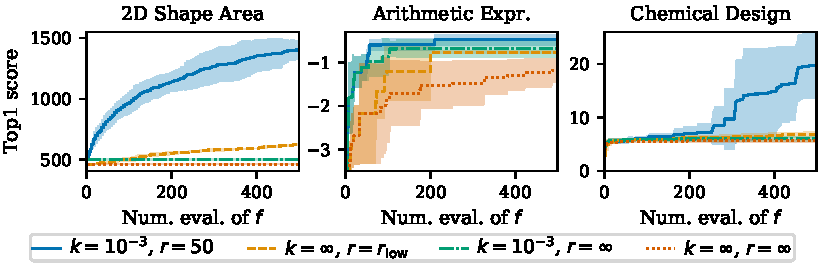
\includegraphics{optimization-top1.pdf}
    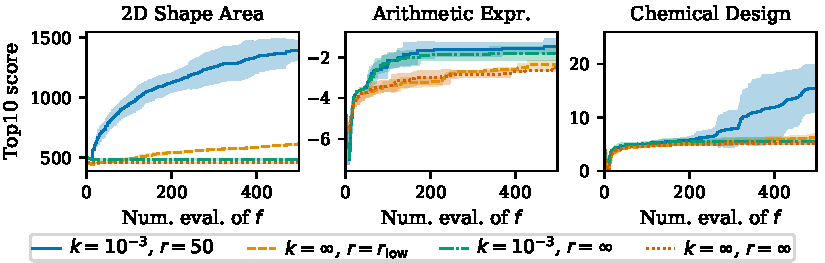
\includegraphics{optimization-top10.pdf}
    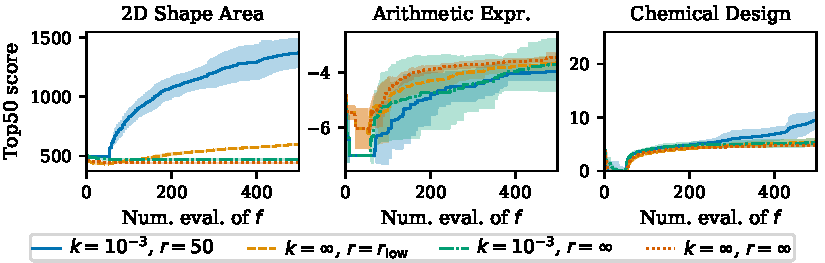
\includegraphics{optimization-top50.pdf}
    \caption[Top$1$, $10$, and $50$ optimisation performance of weighted retraining for all tasks.]{
        Top$1$, $10$, and $50$ optimisation performance of weighted retraining for all tasks,
        for different $k$ values (i.e.\@ $k \in \{10^{-3}, \infty\}$)
        and retraining frequencies (i.e.\@ $r_\text{low} = 5$ for the 2D shape area task,
        and $r_\text{low} = 50$ for the other two tasks). Shaded area corresponds to standard deviation.
    }
    \label{fig:wr-params}
\end{figure}


\subsection{Comparison with Other Methods}
\label{subsec:expt-baselines}
Finally, we compare our proposed method of \gls{lmo} (with weighted retraining) with other methods on the same tasks.
The first class of methods are based on the cross-entropy method as discussed in \cref{sec:lso:related-work},
namely design by adaptive sampling (DbAS) \citep{Brookes_Listgarten_2020},
the cross-entropy method with probability of improvement (CEM-PI) \citep{rubinstein_cross-entropy_1999},
the feedback VAE (FBVAE) \citep{gupta_feedback_2019} and reward-weighted regression (RWR)
\citep{peters2007reinforcement}.
These methods are noteworthy because they can be viewed as a particular case of weighted retraining,
where the weights are binary (except for DbAS)
and the latent optimiser simply consists of sampling from the \gls{dgm}'s prior.
The hyperparameters of these methods are the sequence of quantiles, and the retraining frequency.
We optimise these hyperparameters using a grid search.

\Cref{fig:baselines} shows the performance of these methods on the best hyperparameter setting found, as a function of the number of samples drawn (with a budget of 5,000 samples in total).
We plot the average and standard deviation across 3 random seeds, as we found the variances to be relatively low.
We observe that all other forms of weighted retraining perform significantly worse than our own,
failing to achieve the performance of our approach, even with an evaluation budget that is an order of magnitude larger than ours (i.e.\@ 5,000 vs 500).
We attribute this both to their binary weighting scheme and their lack of a sample-efficient latent optimiser.

\begin{figure}[htb]
    \centering
    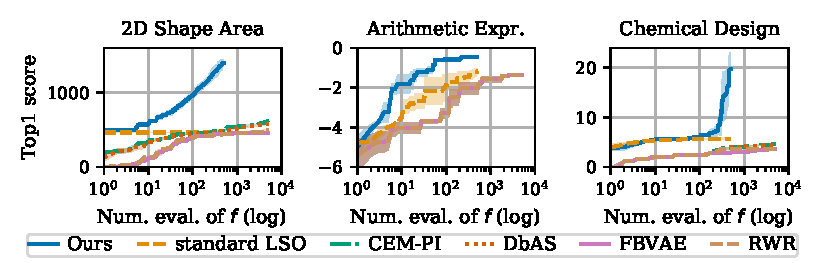
\includegraphics[width=\textwidth]{baselines.pdf}
    \caption[Comparison of weighted retraining, LSO, CEM-PI, DbAS, FBVAE and RWR.]{
        Comparison of weighted retraining, LSO, CEM-PI, DbAS, FBVAE and RWR.
        Our weighted retraining approach significantly outperforms all baselines, achieving both better sample-efficiency and final performance.
    }
    \label{fig:baselines}
\end{figure}

Secondly, we compare against other methods in the literature that have attempted the same chemical design task.
To our knowledge, the best previously reported score obtained using a machine learning method is 11.84 and was obtained with $\approx5000$ samples \citep{zhou_optimization_2019}.
By contrast, our best score is \bestchemscore{} and was achieved with only 500 samples.
Expanding the scope to include more domain-specific optimisation methods,
we acknowledge that ChemBO achieved an impressive score of 18.39 in only 100 samples \citep{korovina2020chembo},
which is better than our method's performance with only 100 samples.
\Cref{tab:chem-results} gives a more detailed comparison with other work.
\Cref{fig:best-molecule-pix} illustrates some of the best molecules found with weighted retraining.
Note that all the high-scoring molecules are extremely large.
It has been reported previously that larger molecules achieve higher scores,
thereby diminishing the impressiveness of this particular design task for \gls{rl} algorithms \citep{zhou_optimization_2019}.
However, the fact that these molecules were found with a generative model strongly highlights
the ability of weighted retraining to find solutions outside of the original training distribution.

\begin{table}[h]
  \centering
  \begin{tabular}{lllll}
    \toprule
    \textbf{Model}     & \textbf{1st}     & \textbf{2nd} & \textbf{3rd} & \textbf{no.\@ queries } \\
    \midrule
    JT-VAE \citep{jin_junction_2019} & 5.30  & 4.93 & 4.49 & $2500^\dagger$     \\
    GCPN \citep{you_graph_2018}     & 7.98 & 7.85 & 7.80 & $\approx10^{6\ddagger}$     \\
    MolDQN \citep{zhou_optimization_2019} & 11.84 & 11.84 & 11.82 & $\geq5000^*$  \\
    ChemBO \citep{korovina2020chembo} & 18.39 & - & - & \textbf{100}$^{**}$ \\
    \midrule
    \textbf{JT-VAE} (our Bayesian optimisation) & 5.65 & 5.63 & 5.43 & 500 \\
    \textbf{JT-VAE} ($k=10^{-3}$, no retraining) & 5.95 & 5.75 & 5.72 & 500 \\
    \textbf{JT-VAE} ($k=10^{-3}$, retraining) & 21.20 & 15.34 & 15.34 & 500 \\
    \textbf{JT-VAE} ($k=10^{-3}$, retraining, \emph{best result}) & \textbf{27.84} & \textbf{27.59} & \textbf{27.21} & \textbf{500} \\
    \bottomrule
  \end{tabular}
  \caption[Comparison of top 3 scores on chemical design task.]{
    Comparison of top 3 scores on chemical design task.
  Baseline results are copied from \citep{zhou_optimization_2019}.
  All our results state the \emph{median} of 5 runs unless otherwise stated (judged by best result),
  each run being 500 epochs.
  $^\dagger$These were the top results across 10 seeds, with 250 queries performed per seed.
  $^\ddagger$Obtained through email correspondence with the authors.
  $^*$The experimental section states that the model was trained for 5000 episodes,
  so at least 5000 samples were needed.
  It is unclear if any batching was used, which would make the number of samples greater.
  $^{**}$From table 3 of \citet{korovina2020chembo}.
  }
  \label{tab:chem-results}
\end{table}

\begin{figure}[ht]
    \centering
    \begin{tikzpicture}
        \draw (0, 0) node[inner sep=0] {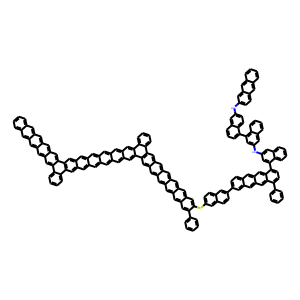
\includegraphics[width=0.3\linewidth]{{mol_pictures/mol_27.84}.png}};
        \draw (0, 1) node {27.84};
    \end{tikzpicture}
    \begin{tikzpicture}
        \draw (0, 0) node[inner sep=0] {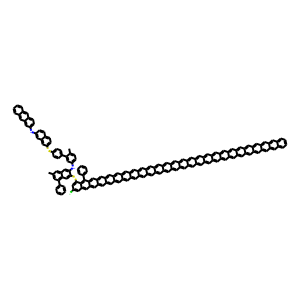
\includegraphics[width=0.3\linewidth]{{mol_pictures/mol_27.59}.png}};
        \draw (1, 1) node {27.59};
    \end{tikzpicture}
    \begin{tikzpicture}
        \draw (0, 0) node[inner sep=0] {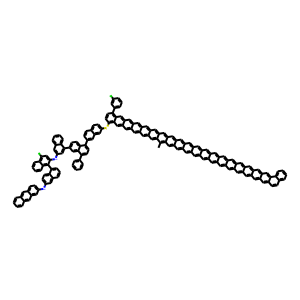
\includegraphics[width=0.3\linewidth]{{mol_pictures/mol_27.21}.png}};
        \draw (1, 1) node {27.21};
    \end{tikzpicture}
    \begin{tikzpicture}
        \draw (0, 0) node[inner sep=0] {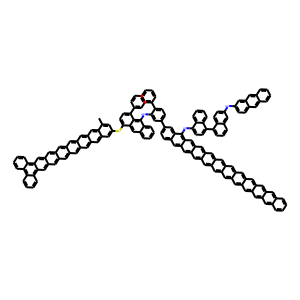
\includegraphics[width=0.3\linewidth]{{mol_pictures/mol_25.90}.png}};
        \draw (1, 1) node {25.90};
    \end{tikzpicture}
    \begin{tikzpicture}
        \draw (0, 0) node[inner sep=0] {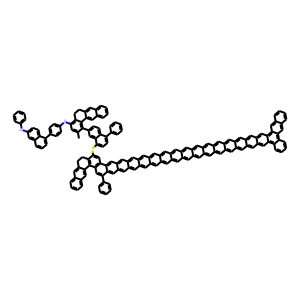
\includegraphics[width=0.3\linewidth]{{mol_pictures/mol_25.37}.png}};
        \draw (1, 1) node {25.37};
    \end{tikzpicture}

    \caption[Molecules found by LSO with logP scores.]{Some of the best molecules for the logP maximisation task found using weighted retraining. Numbers indicate the logP score of each molecule.}
    \label{fig:best-molecule-pix}
\end{figure}

\section{Discussion}
\label{sec:lso:conclusion}
We proposed a method for efficient black-box optimisation over high-dimensional, structured input spaces, combining latent space optimisation with weighted retraining.
We showed that while being conceptually simple and easy to implement on top of previous methods, weighted retraining significantly boosts their efficiency and performance on challenging real-world optimisation problems.

There are several drawbacks to our method that are promising directions for future work.
Firstly, we often found it difficult to train a latent objective model that performed well at optimisation in the latent space, which is critical for good performance.
We believe that further research is necessary into other techniques to make the latent space of \glspl{dgm}
more amenable to optimisation.
Secondly, our method requires a large dataset of labelled data to train a \gls{dgm},
making it unsuitable for problems with very little data,
motivating adaptations that would allow unlabelled data to be utilized.
Finally, due to being relatively computationally intensive, we were unable to characterize
the long-term optimisation behaviour of our algorithm.
In this regime, we suspect that it may be beneficial to use a weighting \emph{schedule}
instead of a fixed weight, which may allow balancing exploration vs.\@ exploitation similar to simulated annealing \citep{van1987simulated}.
Overall, we are excited about the potential results of \gls{lmo} and hope that it can be applied to a variety of real-world problems in the near future.


\section{Retrospective}

Since the publication of this chapter over three years ago
as \citet{tripp2020sample},
it has gone on to be my single most-cited work
(over 100 citations as of February 2024 according to Google Scholar).
Most papers citing \citet{tripp2020sample}
simply refer to it for the term ``latent space optimisation'',
or as one approach out of many for optimising molecular properties.
A few works do notably build upon these ideas though.
\citet{stanton2022accelerating} uses rank-based weights to sample
protein sequences in a similar latent-space BO algorithm.
\citet{lee2023advancing} and \citet{maus2022local} both train
a surrogate model $h:\Z\mapsto\R$ \emph{jointly} with the generative model,
whereas in this work it was still fit afterwards.
\citet{maus2022local} and \citet{notin2021improving} both propose methods
to better-define the optimisation bounds within $\Z$ to avoid
out-of-distribution latent inputs.
Overall, this work has clearly prompted interest in latent space optimisation
methods and inspired follow-up works.

Despite this, I am currently pessimistic about the potential of \gls{lmo}
methods to be highly useful for molecule discovery.
There are two main reasons for this.
First, all of these works required large labelled datasets for some part of the algorithm,
despite many molecule discovery tasks having very few labelled data points.
Although in principle one could apply any of these methods with smaller datasets,
it is very likely that using smaller datasets would lead to overfitting
(I observed this in my own experiments performed after the publication of \citet{tripp2020sample}).
Second, although there may not be a lot of kernels available for arbitrary structured inputs,
graph- and molecule-structured inputs are well-studied and there are many kernels
available for such inputs (see~\S\ref{sec:background:gps}).
Unlike kernels produced via a latent space,
established graph kernels are likely to be more interpretable and 
vary ``smoothly'' with respect to molecular structure.
My opinion is that, in low-data settings, established graph kernels will
generally induce a more sensible prior over objective functions.
